\pdfminorversion=4
\documentclass[aspectratio=169]{beamer}

\mode<presentation>
{
  \usetheme{default}
  \usecolortheme{default}
  \usefonttheme{default}
  \setbeamertemplate{navigation symbols}{}
  \setbeamertemplate{caption}[numbered]
  \setbeamertemplate{footline}[frame number]  % or "page number"
  \setbeamercolor{frametitle}{fg=white}
  \setbeamercolor{footline}{fg=black}
} 

\usepackage[english]{babel}
\usepackage[utf8x]{inputenc}
\usepackage{tikz}
\usepackage{courier}
\usepackage{array}
\usepackage{bold-extra}
\usepackage{minted}
\usepackage[thicklines]{cancel}
\usepackage{fancyvrb}

\xdefinecolor{dianablue}{rgb}{0.18,0.24,0.31}
\xdefinecolor{darkblue}{rgb}{0.1,0.1,0.7}
\xdefinecolor{darkgreen}{rgb}{0,0.5,0}
\xdefinecolor{darkgrey}{rgb}{0.35,0.35,0.35}
\xdefinecolor{darkorange}{rgb}{0.8,0.5,0}
\xdefinecolor{darkred}{rgb}{0.7,0,0}
\definecolor{darkgreen}{rgb}{0,0.6,0}
\definecolor{mauve}{rgb}{0.58,0,0.82}

\title[2011-11-30-acat-python-cpp]{Lessons learned in Python-C++ integration}
\author{Jim Pivarski}
\institute{Princeton University -- IRIS-HEP}
\date{December 1, 2021}

\usetikzlibrary{shapes.callouts}

\begin{document}

\logo{\pgfputat{\pgfxy(0.11, 7.4)}{\pgfbox[right,base]{\tikz{\filldraw[fill=dianablue, draw=none] (0 cm, 0 cm) rectangle (50 cm, 1 cm);}\mbox{\hspace{-8 cm}
\includegraphics[height=1 cm]{princeton-logo-long.png}\hspace{0.1 cm}\raisebox{0.1 cm}{
\includegraphics[height=0.8 cm]{iris-hep-logo-long.png}}\hspace{0.1 cm}}}}}

\begin{frame}
  \titlepage
\end{frame}

\logo{\pgfputat{\pgfxy(0.11, 7.4)}{\pgfbox[right,base]{\tikz{\filldraw[fill=dianablue, draw=none] (0 cm, 0 cm) rectangle (50 cm, 1 cm);}\mbox{\hspace{-8 cm}
\includegraphics[height=1 cm]{princeton-logo.png}\hspace{0.1 cm}\raisebox{0.1 cm}{
\includegraphics[height=0.8 cm]{iris-hep-logo.png}}\hspace{0.1 cm}}}}}

% Uncomment these lines for an automatically generated outline.
%\begin{frame}{Outline}
%  \tableofcontents
%\end{frame}

% START START START START START START START START START START START START START

\begin{frame}{\mbox{ }}
\Large

\vspace{0.5 cm}
This talk is about \textcolor{darkblue}{lessons learned in Python-C++ integration}.

\vspace{1.5 cm}
Awkward Array is the case study.

\vspace{0.25 cm}
\begin{center}

\includegraphics[width=0.35\linewidth]{awkward-logo.pdf}
\end{center}
\end{frame}

\begin{frame}{What is Awkward Array?}
\large
\vspace{0.25 cm}

Efficient representation of variable length, nested, JSON-like data with NumPy-like functions to quickly compute and restructure data in Python.

\begin{columns}
\column{1.15\linewidth}
\only<1>{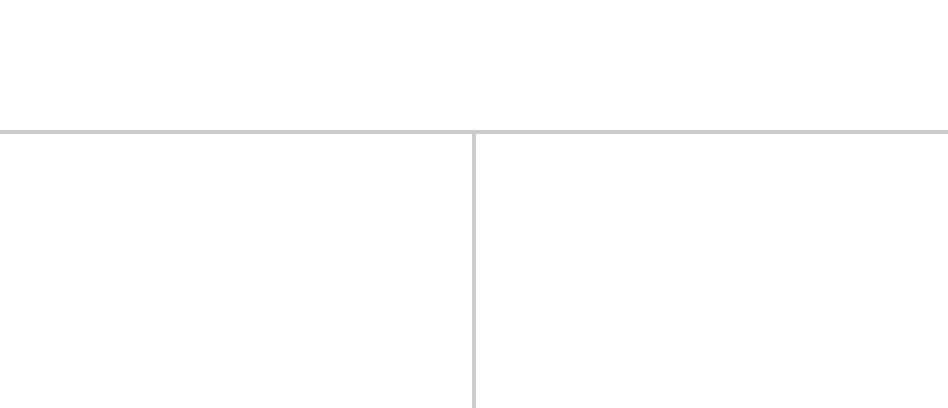
\includegraphics[width=\linewidth]{pivarski-one-slide-summary-0.pdf}}\only<2>{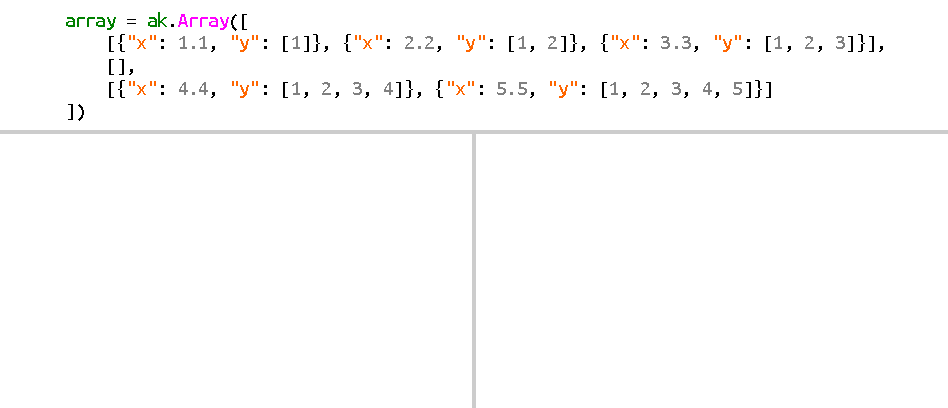
\includegraphics[width=\linewidth]{pivarski-one-slide-summary-1.pdf}}\only<3>{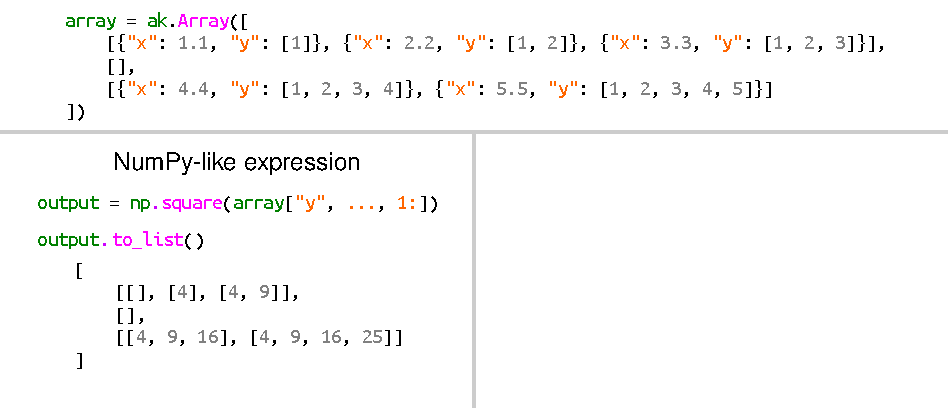
\includegraphics[width=\linewidth]{pivarski-one-slide-summary-2.pdf}}\only<4>{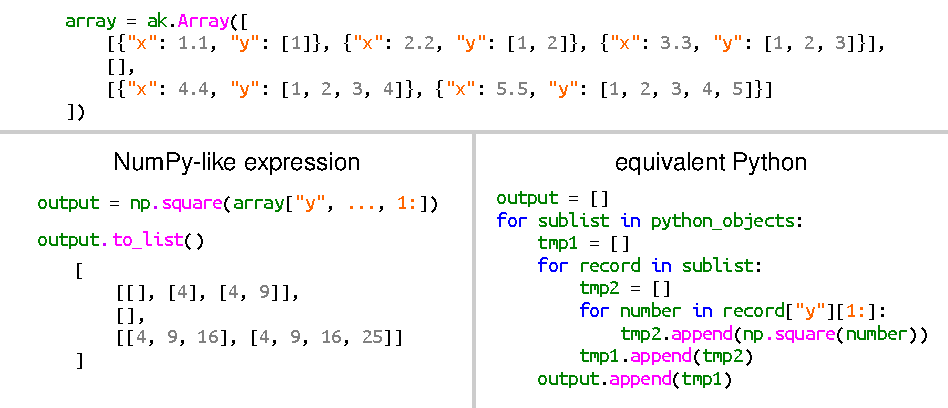
\includegraphics[width=\linewidth]{pivarski-one-slide-summary-3.pdf}}
\end{columns}
\end{frame}

\begin{frame}{History of the project}

\begin{columns}
\column{1.15\linewidth}
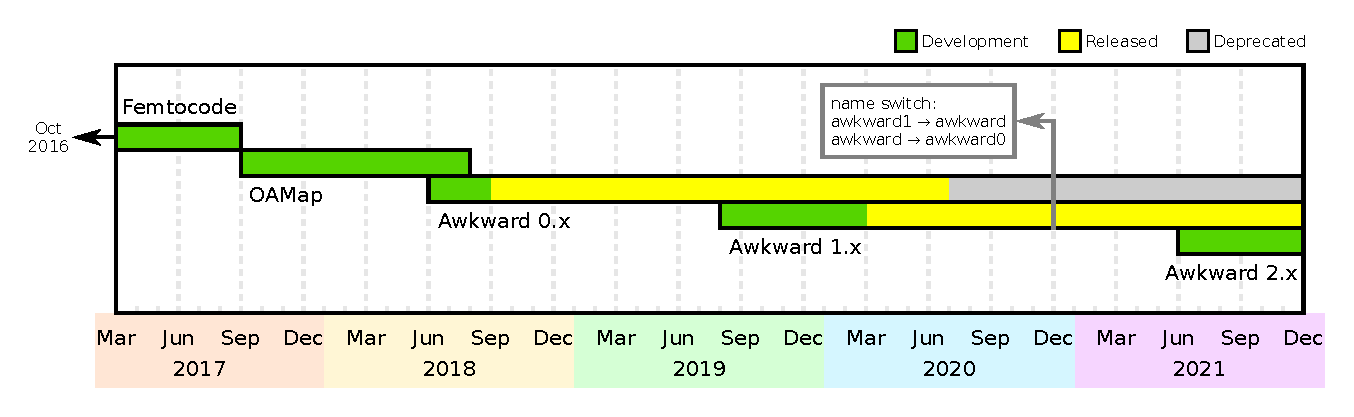
\includegraphics[width=\linewidth]{awkward-timeline.pdf}
\end{columns}

\begin{uncoverenv}<2->
\begin{itemize}
\item Prehistory: Femtocode {\small (\textcolor{darkgreen}{21 kLOC Python})} and OAMap {\small (\textcolor{darkgreen}{8 kLOC Python})}
\item Awkward 0.x: first users, first API, pure Python + NumPy {\small (\textcolor{darkgreen}{9 kLOC Python})}
\item Awkward 1.x: rewrite for stability \& API \mbox{\small (\textcolor{darkgreen}{22 kLOC Python}, \textcolor{blue}{70 kLOC C++}, \textcolor{violet}{14 kLOC C})\hspace{-0.5 cm}}
\item Awkward 2.x: refactor for maintainability \mbox{\small (\textcolor{darkgreen}{29 kLOC Python}, \textcolor{blue}{10 kLOC C++}, \textcolor{violet}{9 kLOC C})\hspace{-0.5 cm}}
\end{itemize}
\end{uncoverenv}
\end{frame}

\begin{frame}{Language changes}
\large
\vspace{0.5 cm}

\textcolor{darkblue}{Awkward 0.x $\to$ 1.x:} complete rewrite with the intention of changing the API.

\vspace{0.25 cm}
Also had to replace some NumPy function calls with precompiled C functions, so we built the infrastructure in C++ with Python only for the high-level front-end.

\vspace{1 cm}
\begin{uncoverenv}<2->
\textcolor{darkblue}{Awkward 1.x $\to$ 2.x:} we are now porting the C++ infrastructure back to Python.

\vspace{0.25 cm}
(For reasons described later in this talk.)

\vspace{0.25 cm}
\begin{center}
\begin{tabular}{c r r}
\textcolor{darkgreen}{Python} & \textcolor{darkgreen}{$-19.6$~kLOC} & \textcolor{darkgreen}{$+26.9$~kLOC} \\
\textcolor{blue}{C++} & \textcolor{blue}{$-59.8$~kLOC} & \textcolor{blue}{$+0$~kLOC} \\
\textcolor{violet}{C} & \textcolor{violet}{$-4.9$~kLOC} & \textcolor{violet}{$+0$~kLOC} \\
\end{tabular}

\vspace{0.25 cm}
\textcolor{gray}{\scriptsize kLOC = thousands of non-blank, non-comment lines of code counted by \mintinline{bash}{cloc}}

\textcolor{gray}{\scriptsize Awkward 2.x is 75\% done; the above is a projection}
\end{center}
\end{uncoverenv}
\end{frame}

\begin{frame}{Evolution of architecture: Awkward \only<1>{0.x}\only<2>{1.x}\only<3>{2.x}}
\vspace{0.25 cm}
\begin{columns}
\column{1.15\linewidth}
\mbox{\hspace{1 cm}\only<1>{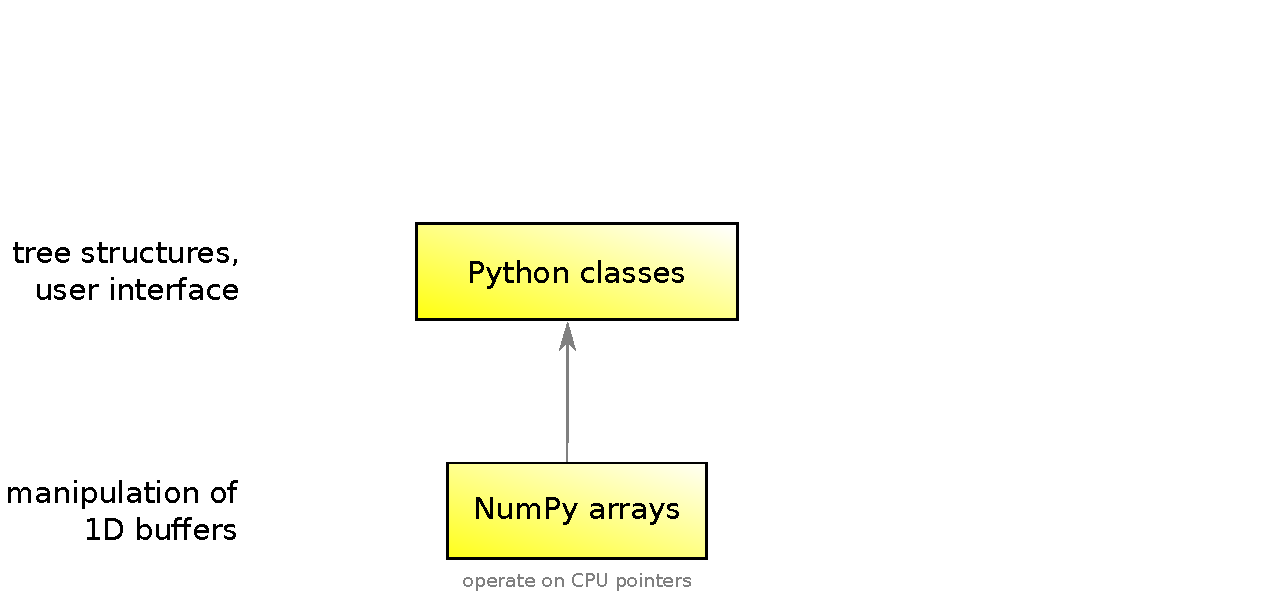
\includegraphics[width=\linewidth]{awkward-0-layers.pdf}}\only<2>{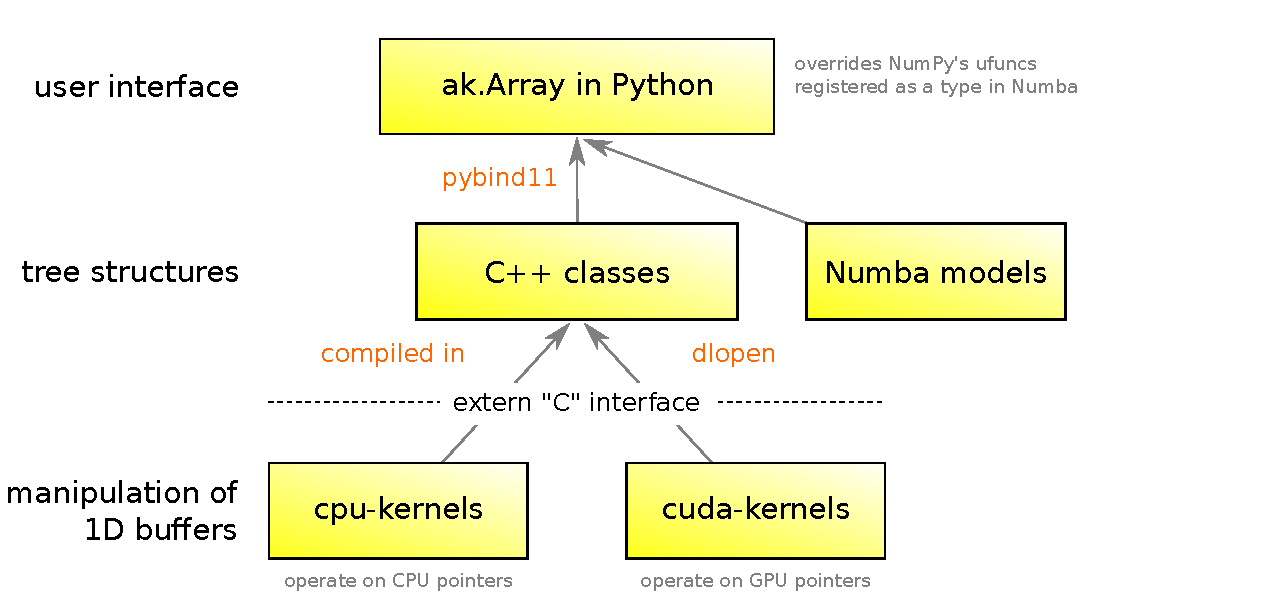
\includegraphics[width=\linewidth]{awkward-1-layers.pdf}}\only<3>{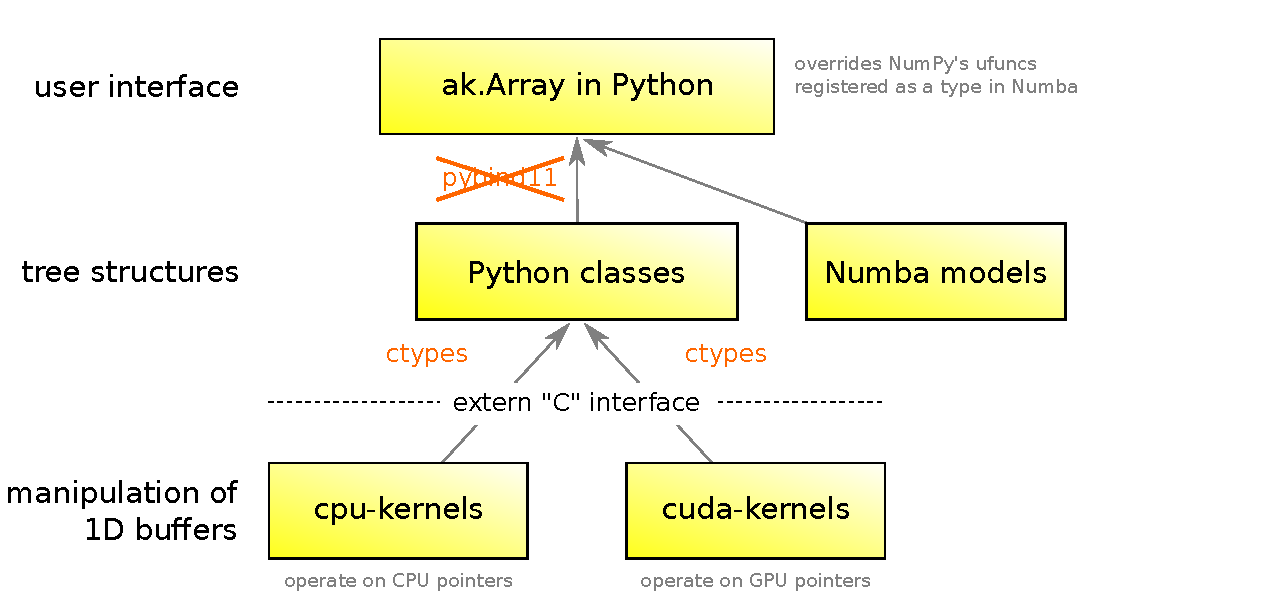
\includegraphics[width=\linewidth]{awkward-2-layers.pdf}}}
\end{columns}
\end{frame}

\begin{frame}{This language choice is unrelated to performance}
\large

\vspace{0.25 cm}
All $\mathcal{O}(n)$ operations for arrays of length $n$ are performed in the kernels layer (C).

\vspace{0.15 cm}
Porting the tree structures from C++ to Python has no $\mathcal{O}(n)$ impact.

\vspace{0.15 cm}
\begin{uncoverenv}<2->
\mbox{ } \hfill \textcolor{darkblue}{For an array of 30~million lists of records:} \hfill \mbox{ }

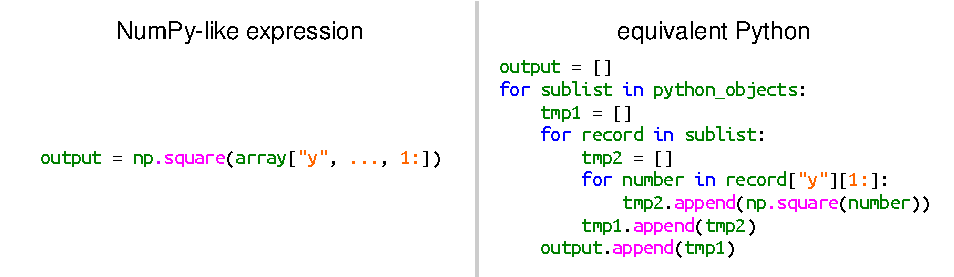
\includegraphics[width=\linewidth]{numpy-like-vs-equivalent-python.pdf}

\vspace{0.25 cm}
\begin{columns}
\column{0.37\linewidth}
Awkward 0.15.5: \hfill\textcolor{darkblue}{4.6~seconds}

Awkward 1.5.1: \hfill\textcolor{darkblue}{2.4~seconds}

Awkward 2.0.0a: \hfill\textcolor{darkblue}{1.5~seconds}

\column{0.4\linewidth}
equivalent Python: \textcolor{darkblue}{140~seconds}

\textcolor{gray}{because $\mathcal{O}(n)$ operations are performed in Python}
\end{columns}
\end{uncoverenv}
\end{frame}

\begin{frame}{\mbox{ }}
\LARGE
\begin{center}
\textcolor{darkblue}{Lessons learned in Python-C++ integration}
\end{center}
\end{frame}

\begin{frame}{Issue \#1: Intention to use C++ as an ABI}
\large

\vspace{0.5 cm}
Awkward 1.x design goal: connect to C++ HEP libraries through the C++ layer.

\vspace{0.25 cm}
Awkward 2.x removes this capability.

\vspace{0.25 cm}
\begin{itemize}\setlength{\itemsep}{0.25 cm}
\item<2-> Python packages must be distributed as binaries, with compilation-on-install {\it as a last resort!} ``\mintinline{bash}{pip install awkward}'' shouldn't have dependencies outside of \mintinline{bash}{pip}, including the existence of a compiler.

\item<3-> Dynamically linking to precompiled C++ exposes a project to ABI dependencies. Awkward-enabled HEP libraries would depend on ABI version.

{\scriptsize (See \mintinline{bash}{PYBIND11_INTERNALS_VERSION} in \mintinline{bash}{pybind11/include/pybind11/detail/internals.h}.)}

\item<4-> \textcolor{darkorange}{\bf Not needed anyway:} \textcolor{blue}{\href{https://github.com/scikit-hep/fastjet}{fastjet}}, a Python/Awkward interface to \mbox{\textcolor{blue}{\href{http://fastjet.fr/}{FastJet}} (C++),\hspace{-0.5 cm}} interfaces through C data types (raw arrays) easily.

\vspace{0.25 cm}
Awkward Array does not need to be C++ to

interface with C++.
\end{itemize}

\vspace{-1.65 cm}
\hfill \uncover<4->{
\includegraphics[width=0.3\linewidth]{fastjet-logo.pdf}}

\vspace{-0.15 cm}
\hfill \uncover<4->{{\small See Aryan Roy's poster!} \hspace{0.2 cm}}
\end{frame}

\begin{frame}{Issue \#2: Reference cycles through C++}
\vspace{0.15 cm}

\begin{columns}
\column{1.16\linewidth}
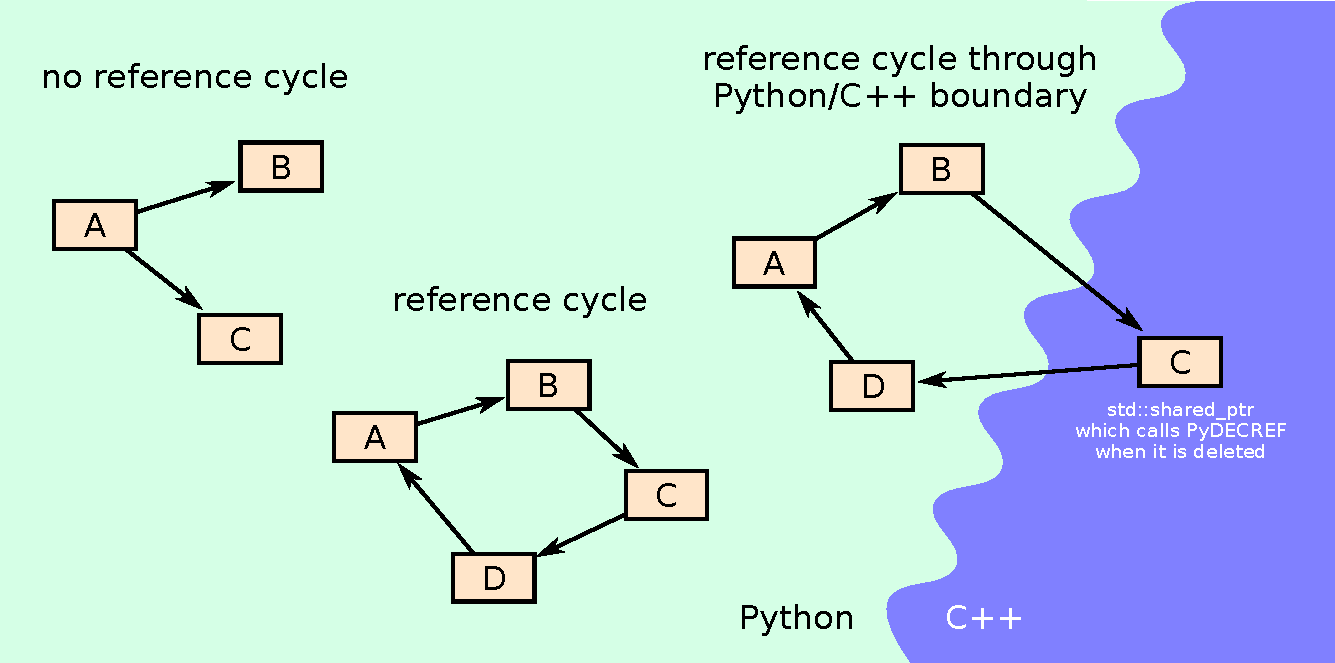
\includegraphics[width=\linewidth]{python-cpp-reference-cycles.pdf}
\end{columns}
\end{frame}

\begin{frame}{Issue \#2: Reference cycles through C++}
\large
\vspace{0.25 cm}
\begin{itemize}\setlength{\itemsep}{0.15 cm}
\item<1-> In most circumstances, Awkward Arrays have no reference cycles because they're immutable.

\item<2-> VirtualArrays (for lazy evaluation) maintain a cache to avoid repeat evaluations. Sometimes, a VirtualArray is put inside its own cache.

\item<3-> Python garbage collector can detect reference cycles, immediately when a reference count goes to zero or during mark-and-sweep.

\item<4-> But it can't detect a reference cycle through C++.

\item<5-> We tried to fix this by making the VirtualArray cache a weakref, but this had its own share of issues: {\normalsize \#230, \#400, \#432, \#479, \#541, \#560, \#597, \#603, \#655, \#679, \#783, \#865, \#899, \#940, \#1052\ldots}

\item<6-> Even sneakier: reference cycles can be created by function closures; VirtualArrays hold Python functions. (Anything mutable is an opening!)

\item<7-> Dropping C++ solves this, but we're also replacing VirtualArrays with Dask.
\end{itemize}
\end{frame}

\begin{frame}{Issue \#3: Releasing the GIL}
\large
\vspace{0.5 cm}
\hfill 
\includegraphics[height=4 cm]{python-gil-eat-concurrency.jpg}

\vspace{-3.75 cm}
If you're using pybind11, be aware that it does not release

Python's GIL by default. The GIL undermines multithreading.

\vspace{0.25 cm}
{\small \textcolor{gray}{(See \mintinline{c++}{py::gil_scoped_acquire}, \mintinline{c++}{py::gil_scoped_release},}

\textcolor{gray}{and \mintinline{c++}{py::call_guard}.)}}

\vspace{0.5 cm}
\uncover<2->{Furthermore, you can't release the GIL if you ever need to}

\uncover<2->{change any Python object, even a reference counter.}

\vspace{0.5 cm}
\uncover<3->{Awkward Array's C++ objects hold references to Python objects (mostly NumPy arrays) and decrement the reference count if the C++ object is deleted. Since that could happen at any time, we can't release the GIL without risking segfaults.}
\end{frame}

\begin{frame}{Issue \#4: Algorithm visibility}
\large

\vspace{0.25 cm}
The {\it final} reason for C++ $\to$ Python refactoring: third-party libraries like Dask and JAX couldn't ``see'' enough of what Awkward Array was doing.

\only<1>{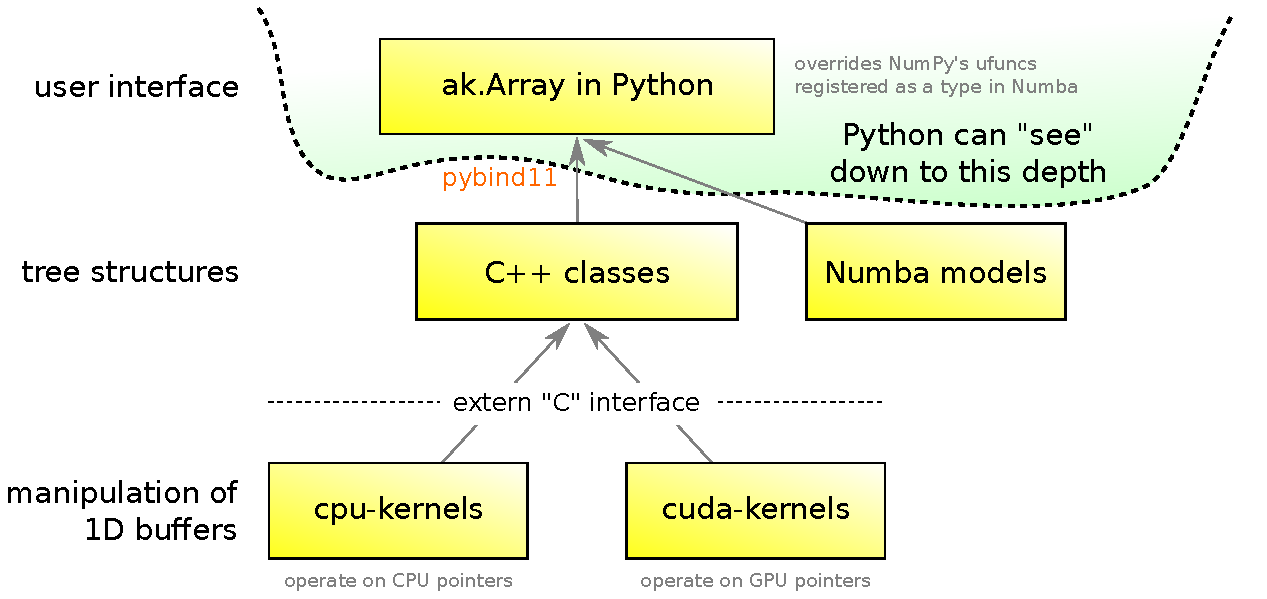
\includegraphics[width=\linewidth]{awkward-1-layers-problem.pdf}}\only<2>{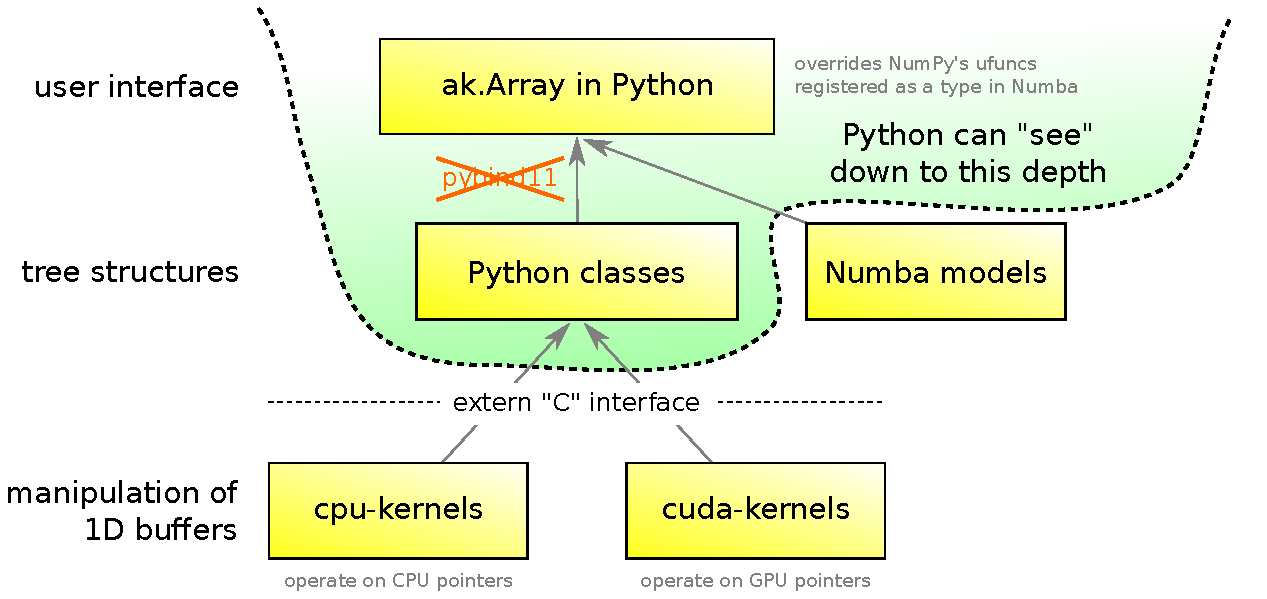
\includegraphics[width=\linewidth]{awkward-2-layers-solution.pdf}}
\end{frame}

\begin{frame}[fragile]{Issue \#4: Algorithm visibility}
\vspace{0.5 cm}

\large
These libraries use ``tracers'' to inspect a path through Python code, like this:

\small
\begin{minted}{python}
>>> import numpy as np
>>> class Tracer(np.lib.mixins.NDArrayOperatorsMixin):
...     def __init__(self):
...         self.functions = []
...     def __array_ufunc__(self, ufunc, method, *inputs, **kwargs):
...         self.functions.append(ufunc.__name__)
...         return self
... 
>>> t = Tracer()
>>> np.sin(t)**2 + np.cos(t)**2
<__main__.Tracer object at 0x7ff2a0f33e80>
>>> t.functions
['sin', 'power', 'cos', 'power', 'add']
\end{minted}

\large
\vspace{0.5 cm}
Tracers can see binary ops and functions, but calls out of Python are black boxes.
\end{frame}

\begin{frame}{Issue \#4: Algorithm visibility}
\large
\vspace{0.5 cm}

The ``tree structures'' (mid-level) of Awkward Array are too coarse for these libraries because the third-party libraries don't recognize arrays of trees.

\vspace{0.5 cm}
They {\it do} recognize simple arrays of numbers (our ``kernels,'' or low-level).

\vspace{0.5 cm}
See Anish Biswas's presentation at \textcolor{blue}{\href{https://indico.cern.ch/event/1033648}{https://indico.cern.ch/event/1033648}} for a heroic attempt to integrate Awkward Array and JAX using PyTrees.

\vspace{0.5 cm}
\uncover<2->{\textcolor{darkorange}{\bf This last problem with Awkward Array's C++ layer is the one that finally convinced us to change.}}
\end{frame}

\begin{frame}{\mbox{ }}
\LARGE
\begin{center}
\textcolor{darkblue}{Awkward Array's Python-C++ codebase was a bad design.}

\vspace{1 cm}
\textcolor{darkblue}{\uncover<2->{Does that mean you shouldn't mix Python and C++?}}
\end{center}
\end{frame}

\begin{frame}{\mbox{ }}
\Huge
\begin{center}
\textcolor{darkblue}{\bf No!}
\end{center}
\end{frame}

\begin{frame}{\mbox{ }}
\vspace{0.25 cm}
\LARGE
\textcolor{darkblue}{Just watch out for these issues when you do.}

\vspace{0.25 cm}
\Large
\begin{enumerate}\setlength{\itemsep}{0.25 cm}
\item Don't plan on sharing stdlib (e.g.\ \mintinline{c++}{std::vector}) or pybind11 objects between Python modules. Share data as basic C types.

\item Python and C++ can share references, but ensure no reference cycles! 100\% immutability would prevent cycles.

\item You can only release the GIL in blocks of code that do not touch Python in any way, including reference counts.

\item Think about interoperability plans: how much of your code will third-party libraries need to see?
\end{enumerate}
\end{frame}

\begin{frame}{\mbox{ }}
\LARGE
\begin{center}
\textcolor{darkblue}{Basically, keep Python and C++ an arm's length apart.}

\Large
\vspace{1 cm}
\textcolor{darkblue}{\uncover<2->{A ``loose coupling'' avoids most of these issues.}}

\normalsize
\vspace{1 cm}
\textcolor{darkblue}{\uncover<3->{(This may be an advertisement for Julia.)}}
\end{center}
\end{frame}

\end{document}

%% Description
%% Awkward Array 0.x was written entirely in Python, and Awkward Array 1.x was a fresh rewrite with a C++ core and a Python interface. Ironically, the Awkward Array 2.x project is translating most of that core back into Python (leaving the interface untouched). This is because we discovered surprising and subtle issues in Python-C++ integration that can be avoided with a more minimal coupling: we can still put performance-critical code in C++, but also benefit by minimizing the interface between the two languages.

%% This talk is intended to share what we learned from our experiences: design choices that look innocent but can cause issues several steps later, often only in the context of real applications. The points to be presented are (1) memory management: although Python references can be glued to std::shared_ptr, cycles through C++ are invisible to Python's garbage collector and can arise in subtle ways, (2) C++ standard library types are not a portable runtime interface, owing to ABI differences, and (3) tracers, at the heart of Python libraries like Dask and JAX, can only be fully leveraged if black-box calls out of Python use basic, universally recognized types: flat arrays, not objects.

%% The goal of this talk is to call out these issues so that other projects mixing Python and C++ can avoid them in the design stage.

%% References
%% The closest match to this talk's content can be found in an IRIS-HEP Analysis Systems group meeting: https://indico.cern.ch/event/1032972/

%% But this talk would be for a wider audience, presenting these issues in a more general way: more like "how to" tips than specific project plans.

%% Significance
%% This talk is not aimed at potential users of Awkward Array, but developers working on other projects that need to mix Python and C++. This need is increasingly relevant as more front-ends use Python, but large-scale processing still needs to have high performance.
